\chapter{Chain Mode Settings:}
The CHAIN setting enables or disables Chain Mode.\\
\fbox{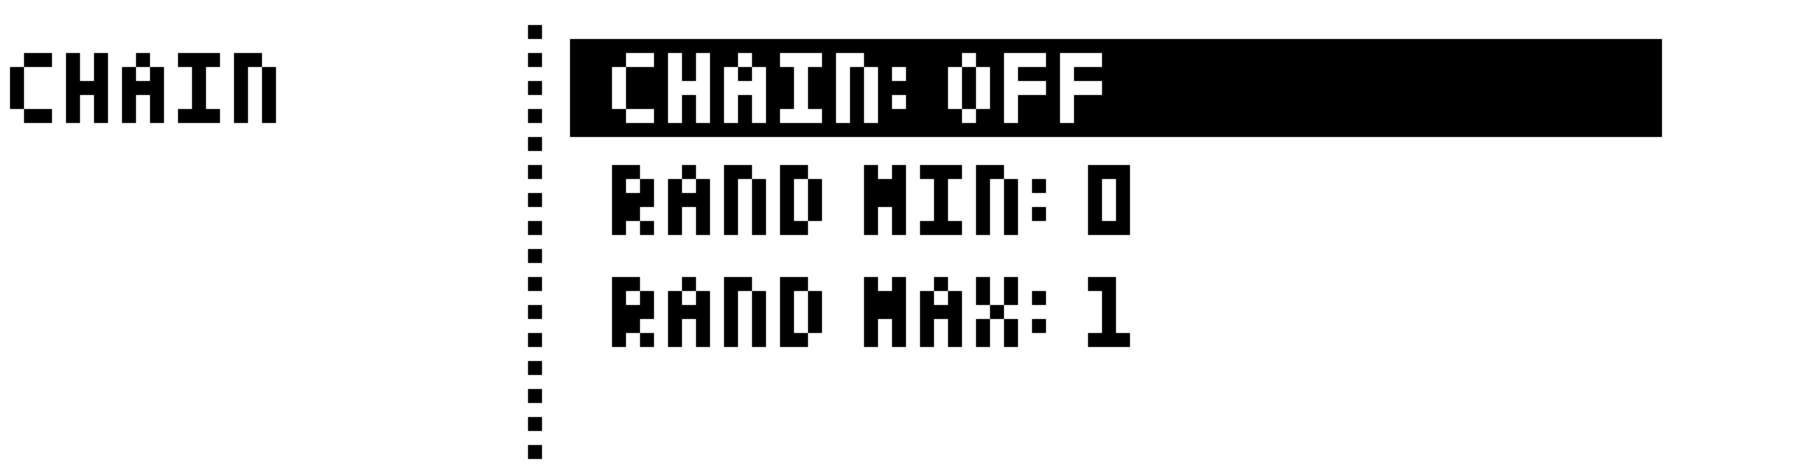
\includegraphics[scale=.40]{chain_menu.png}}\\
\textit{ Chain Mode can be enabled by selecting one of 3 three options: Automatic, Manual and Random.}
\\
\subsection{Chain:}
\begin{itemize}
\item Automatic: If the number of loops is greater than 0, slots will automatically jump to the specified Row after N loops.
\itme Manual: Automatic slot jumping is disabled, but tracks can be chained using the quantization rules in the Chain Page.
Random: Slots will jump after a random number of iterations to a random row position bounded by the min and max settings specified in Global Settings.\\
\itme \subsection{Rand Min/Max:}
The random min + max values are used to specify the minimum + maximum range of rows that will be loaded when random mode is enabled.
\end{itemize}
